\documentclass[
	11pt,
	a4paper
]{scrartcl}

\usepackage[utf8]{inputenc}
\usepackage[ngerman]{babel}
\usepackage[T1]{fontenc}
\usepackage[a4paper]{geometry}
\usepackage{amsmath, amsfonts, amssymb}
\usepackage{color}
\usepackage{graphicx}
\usepackage[headsepline,automark]{scrlayer-scrpage}
\usepackage{blindtext}
\usepackage[hidelinks]{hyperref}
\usepackage{enumitem}\usepackage{float}
\usepackage{soul}
\usepackage[bottom]{footmisc}


% -- CONFIG --
\definecolor{hft}{RGB}{204,49,37}
\setcounter{page}{0} % Do not count first page
\addto\extrasngerman{\def\figureautorefname{Abb.}}
\setlength\parindent{0pt}
\restylefloat{figure}

% -- NEW COMMANDS --
\newcommand{\code}[1]{\texttt{\ul{#1}}}

% -- HEADER --
\pagestyle{scrheadings}
\clearpairofpagestyles
\setkomafont{pageheadfoot}{\upshape}
\ihead{KI Abschlussprojekt (Prof. Dr. Pado)}
\ofoot{Seite \pagemark}


% -- DOCUMENT --
\begin{document}

% -- TITLE PAGE --
\begin{titlepage}
	\makeatletter
  	\begin{center}   
       
\includegraphics[width=0.4\textwidth]{figures/HFT-logo-gross-Aplusheadline.jpg}
       \vspace{2cm}
       
       \textcolor{hft}{\hrule}
       \vspace{0.5cm}
       {\Huge\scshape Abschlussprojekt}
       \vspace{0.5cm}
       \textcolor{hft}{\hrule}
            
       \vspace{2cm}
       {\large Im Fach Künstliche Intelligenz bei Prof. Dr. Pado}
       \vspace{2cm}
       
       
       \begin{flushleft}\quad Aufgabenstellung:\end{flushleft}
       {\large \textbf{Newsgroups}}
       \vspace{1cm}
       
       \begin{flushleft}\quad Teilnehmer:\end{flushleft}
       {\large Jochen Spender}\\\vspace{0.1cm}
       {\large Luca Lissner}\\\vspace{0.1cm}
       {\large Mario Podda}\\\vspace{0.1cm}
       {\large Samuel Maier}
       \vspace{1cm}
       
       \begin{flushleft}\quad Abgabe:\end{flushleft}
       {\large 18. November 2021}
   \end{center}
\end{titlepage}

% -- TABLE OF CONTENTS AND SOURCES --
%\newgeometry{lmargin={2cm},rmargin={2cm},tmargin={2.5cm},bmargin = {2.5cm}, headsep={0.3cm}}
\newgeometry{left=2cm, right=2cm, top=1.2cm, bottom=1.2cm,includehead,includefoot, headsep=0.3cm,footskip=0.3cm,heightrounded}
\tableofcontents
\newpage

%% -- CONTENT --
\section{Dokumentation unseres Vorgehens}
Zu Beginn des Projektes verschafften wir uns über die vorliegenden Daten einen Überblick,
indem wir diese nach Zielklassen farblich getrennt darstellten. (\autoref{fig:texte_grafisch_getrennt})\\
Zudem stellten wir Nachforschungen zu den Daten und deren Herkunft an und versuchten mit Hilfe von kleinen
Skripts und Excel (\autoref{fig:wort_auswertung_excel}), Gemeinsamkeiten in Abhängigkeit zur Zielklasse
herauszufinden. Anhand dieser Erkenntnisse formulierten wir erste Features. Hierbei waren hauptsächlich Mario
und Jochen beteiligt.\\

Anschließend entwickelte Samuel ein Python Skript, dass eine JSON-Datei einließt, Features berechnet und
dann drei Dateien ausgibt, um in Weka weiter zu arbeiten. Bei der anschließenden Implementierung der Features war Luca
maßgeblich beteiligt.\\

In der letzten Phase des Projektes trainierten wir mit den generierten Dateien Modelle in Weka. Hierfür verwendeten wir
unterschiedliche Featurekombinationen und untersuchten auch den Nutzen einzelner Features. Die entstanden Erkenntnisse
verwendeten wir für die Entwicklung weiterer Features. Durch die Verwendung eines gemeinsamen GIT-Repository waren wir
hier alle parallel beteiligt.\\

Für die Implementierung entschieden wir uns für Python, da uns hierfür schon das Werkzeug NLTK, zum einfacheren Verarbeiten
der Texte zur Verfügung stand.\\
Außerdem exportierten wir den Originaldatensatz aus Weka im *.JSON Format, da uns dieses vertrauter und leichter zu verarbeiten
erschien als das *.ARFF Format.


\section{Daten}
Der \emph{20 Newsgroups} Datensatz ist eine Sammlung aus etwas 20.000 Newsgroup Beiträgen, gleichmäßig unterteilt in 20
verschiedene Themen aus den sog. Big Eight\footnote{Die \emph{Big Eight} stehen für folgende acht Bereiche: Computer,
Diskussion, Gesellschaft \& Politik, Wissenschaft, Kultur, Freizeit \& Hobby, News und Sonstiges.}. Aus einem Kommentar
aus dem Original-Datensatz geht hervor, dass der vermeintliche Autor Ken Lang die Daten für sein Projekt \emph{Newsweeder}
zusammentrug.\\
Der Datensatz wird sehr gerne für Experimente mit Techniken des Maschinellen Lernens wie Textklassifizierung und
Textclustering  benutzt.\\
Es gibt verschiedene Versionen des Datensatzes. Diese unterscheiden sich darin welche Informationen aus den originalen
Newsgroup-Texten (E-Mails) verwendet werden. In unserem Datensatz wurden alle Metadaten wie Datum, Empfänger oder Betreff
entfernt, er enthält jeweils nur die tatsächliche Nachricht.\\

Für dieses Projekt erhielten wir einen Teildatensatz von 3370 Instanzen mit Beiträgen aus den Kategorien Raumfahrt,
Computergrafik, Religion und Atheismus. Er enthält folgende drei Features, die erstmal nicht von Weka zum
Lernen benutzt werden können:
\begin{enumerate}[label=\roman*), itemsep=0pt,parsep=0pt]
	\item ID: Numerisch, eine fortlaufende einzigartige Nummer über alle Instanzen
	\item text: String, enthält den entsprechenden Newsgroup Beitrag
	\item group: Nominal, die Kategorie des Textes welche unseren Zielklassen entspricht:
	\begin{enumerate}[label=\arabic*., itemsep=0pt,parsep=0pt, start=0]
		\item Atheismus
		\item Computergrafik
		\item Raumfahrt
		\item Religion
	\end{enumerate}
\end{enumerate}

Beim Analysieren der Daten bemerkten wir recht schnell, dass die Texte aus den Kategorien Atheismus und 
Religion einen ähnlichen Wortschatz besaßen und es sehr schwer werden würde Texte aus diesen beiden Kategorien zu 
klassifizieren.\\

Wir entschieden uns, den Datensatz im Verhältnis 80:10:10 in Trainings-, Entwicklungs- und Testdaten zu trennen. So besaßen
unsere Entwicklungs- und Testdaten mit jeweils 337 Instanzen immer noch genügend Daten um das gelernte Model zuverlässig 
verifizieren zu können.

\section{Features}
Im folgenden eine Auflistung unserer Features. Meist wurden diese im Projektverlauf verbessert, so dass teilweise ähnliche
Versionen verfügbar sind. Auf die letztendlich benutzten Feature und ihre Nutzbarkeit wird im Abschnitt \emph{\nameref{trainingsprozess}}
näher eingegangen.

\subsection{Zeichen zählen}
Beim Durchschauen der Texte kam uns der Gedanke, dass die Textlänge, also die Anzahl an Zeichen eines Textes, ein mögliches Feature
ist, da die Textlänge der eher technischen Texte aus den Kategorien Computergrafik und Raumfahrt oft kürzer ausfielen als die eher
philosophischen Texte aus Religion und Atheismus.\\
Das Feature \code{count chars} zählt daher für jeden Text die Anzahl an Zeichen.\\

Im weiteren Verlauf des Projektes entwickelte sich daraus die Variante \code{count chars ignore whitespace}, welche beim Zählen alle
Leerzeichen unbeachtet lässt. 

\subsection{Wörter zählen}
Ein weiteres Basis Feature, aus dem sich viele weitere Versionen ableiten ließen, war \code{total word count}. Es zählt, aus wie vielen
Wörtern ein Text besteht. Hierbei werden nur echte Wörten beachtet.\\
Davon abgeleitet entwickelte sich das Feature \code{average word length}, dass die durchschnittliche Wortlänge eines Texte berechnet und
\code{max word length}, dass das längste Wort eines Textes sucht.

\subsubsection{Wortdiversität}
Die Feature \code{lexical diversity} entspricht der Wortdiversität und zählt, aus wie vielen unterschiedlichen Wörtern ein Text besteht.\\
Spezifizierend haben wir das Feature \code{lexical diversity nostop} entwickelt, dass Stoppwörter\footnote{Unter \emph{Stoppwörtern}
versteht man sehr häufig auftretende Wörter, die meist keine direkte Relevanz für den Informationsgehalt eines Textes haben} ignoriert. \\

Um die Wortdiversität weiter zu verfeinern, sollten die Wörter vor dem Zählen normalisiert werden. Hierfür verwendeten wir zwei Methoden,
einmal das sog. Stemming im Feature \code{lexical diversity stemmed nostop} und Lemmatizing im Feature \code{lexical diversity lemmatized
nostop}


\subsection{Wörterlisten}
Anhand von verschiedenen Parameter werden aus den Trainingsdaten für jede Kategorie eine Liste mit den häufigsten Wörtern erstellt.\\
Die Feature-Klasse \code{word Presence for} erstellt für alle ermittelten Wörter jeweils ein Feature, indem entweder
\begin{itemize}[itemsep=0pt,parsep=0pt]
	\item das Vorkommen des Wortes im Text gezählt wird.
	\item das Vorkommen des Wortes in Abhängigkeit mit der Wortanzahl des Text berechnet wird.
	\item das Vorkommen des Wortes in Abhängigkeit der normierten (in diesem Fall gestemmten) Wortanzahl des Textes berechnet wird.
\end{itemize}

Der Parameter \code{takeToByCat} definiert die Anzahl an Wörtern pro Kategorie, für die ein Feature erstellt werden soll, wobei dies noch
durch den Parameter \code{cutOff} beschränkt werden kann, indem nur Wörter gesucht werden die im Verhältnis zu den anderen Kategorien 
häufiger vorkommen.


\section{Trainingsprozess \& Fazit}\label{trainingsprozess}
Im Laufe des Projektes ließen wir Weka mit den verschiedensten Feature Kombinationen trainieren. Anhand der jeweiligen Ergebnisse
veränderten wir bestehende oder entwickelten neue Features.\\






\newpage
\section{Anhang}

\begin{figure}[H]
	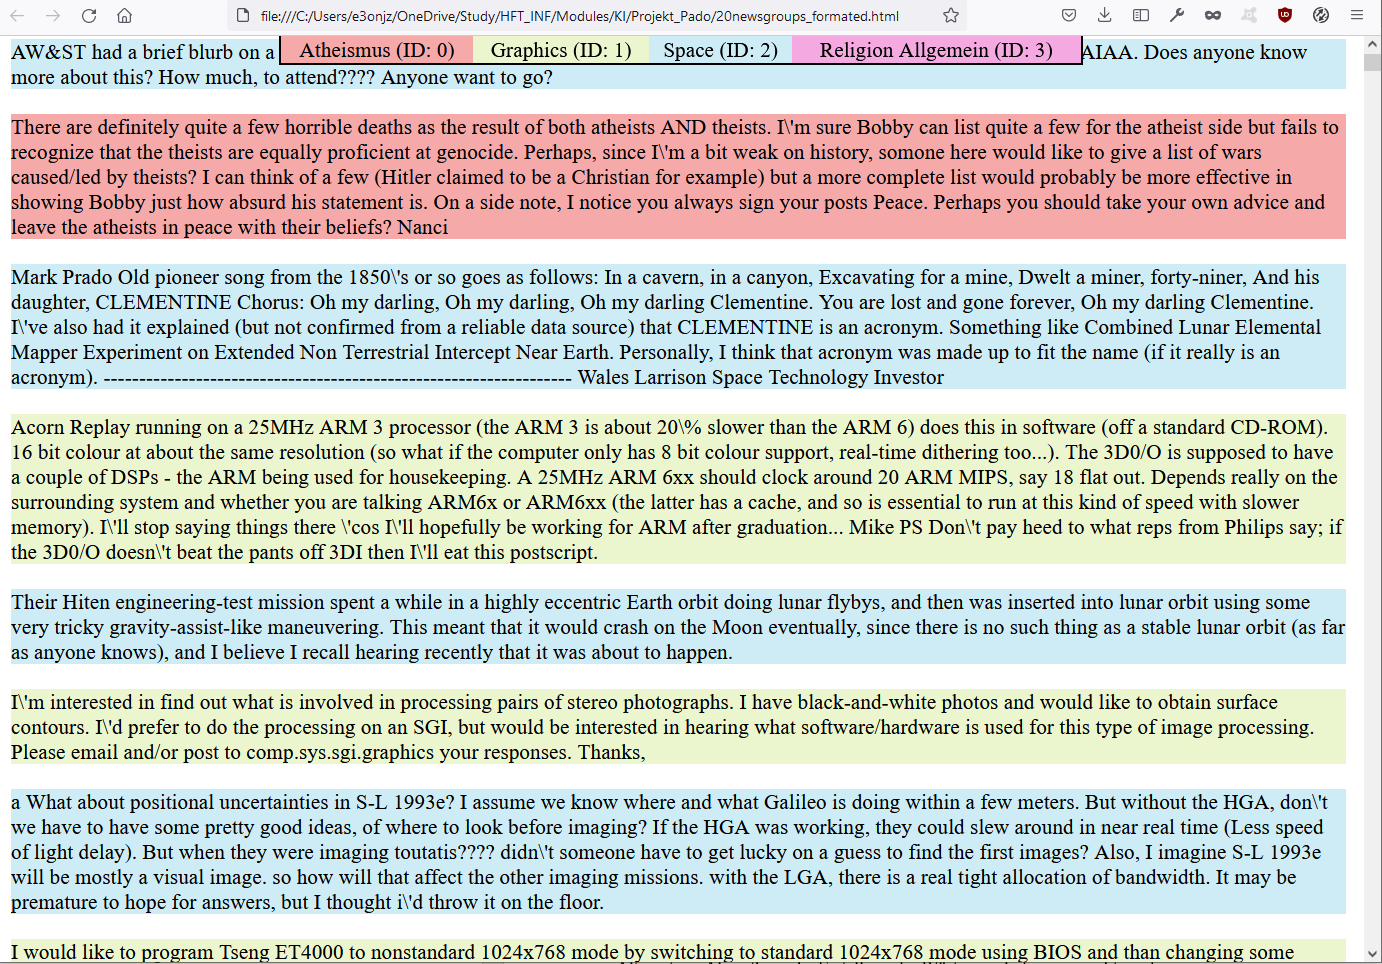
\includegraphics[width=\textwidth]{figures/texte_grafisch_getrennt.png}
	\caption{Texte grafisch nach Kategorie hervorgehoben}
	\label{fig:texte_grafisch_getrennt}
\end{figure}

\begin{figure}[H]
	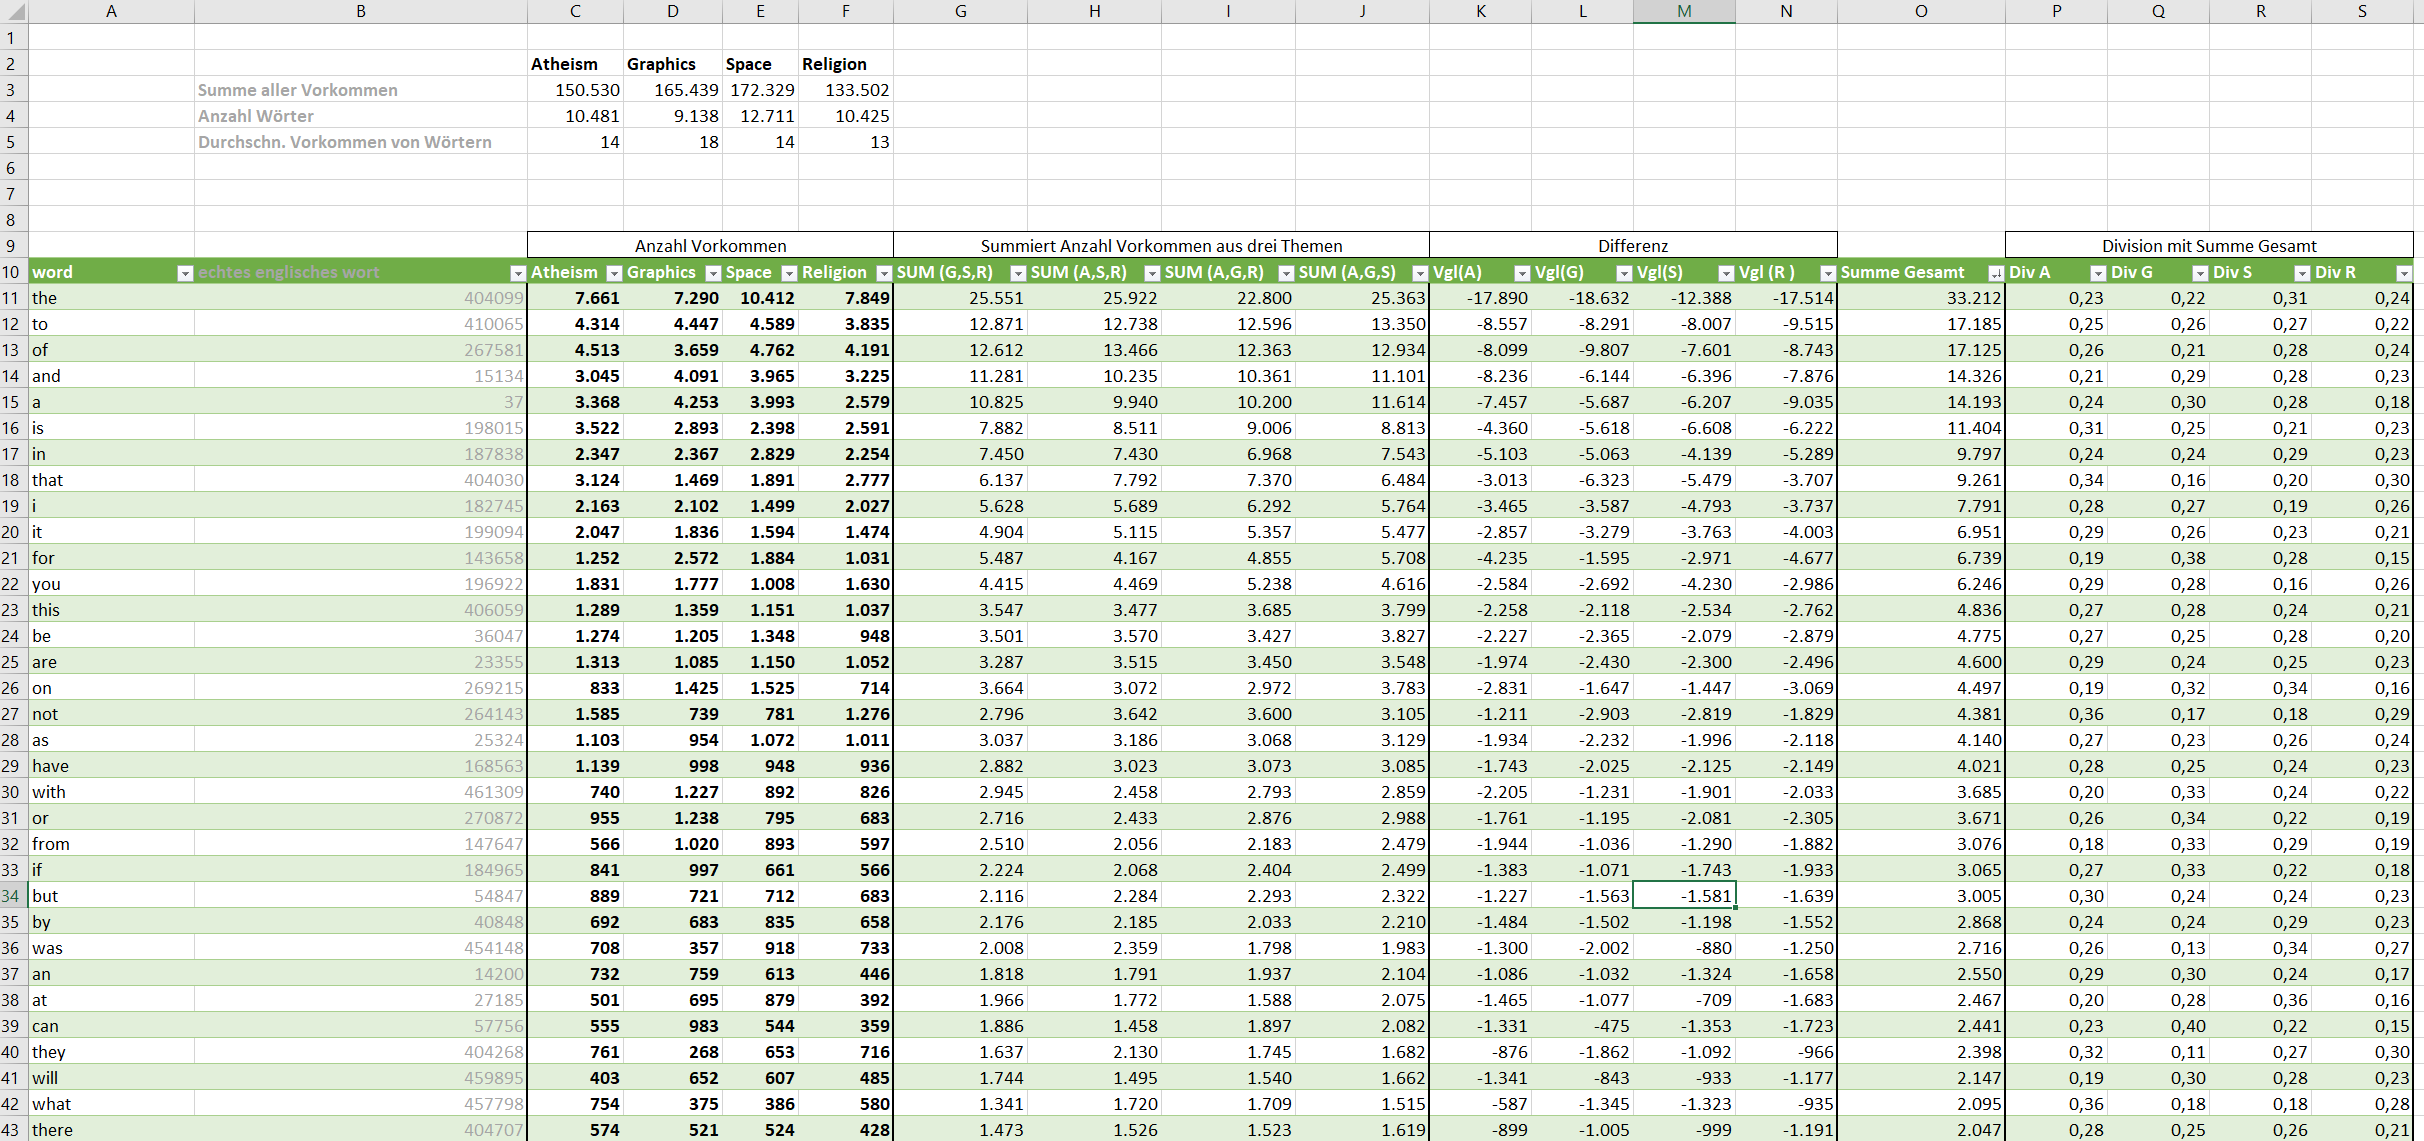
\includegraphics[width=\textwidth]{figures/wort_auswertung_excel.png}
	\caption{Erste Auswertungen über vorkommende Wörter}
	\label{fig:wort_auswertung_excel}
\end{figure}


\end{document}
